\documentclass[12pt,a4paper]{article}
\usepackage[utf8]{inputenc}
\usepackage[T1]{fontenc}
\usepackage[ngerman]{babel}
\usepackage{amsmath}
\usepackage{amsfonts}
\usepackage{amssymb}
\usepackage{graphicx}
\usepackage{packets}
\author{Lars Döpper}
\date{\today}
\title{441 Computerphysik - Hausaufgabe 2}

\begin{document}
	\maketitle
\section{Aufgabe H4 - Gedämpfte Oszillation}
\subsection{Teilaufgabe 1 - Euler-Cauchy-Verfahren}
Wir betrachten zunächst das Euler-Cauchy-Verfahren für diese Differentialgleichung. Wir bringen dazu als Erstes die Differentialgleichung auf vektorielle Form. Diese lautet dann:
\begin{equation}
	\vec{f}(t) = \dot{\vec{x}} = \begin{pmatrix} \dot{x^{(1)}} \\ \dot{x^{(2)}}	\end{pmatrix} = 
	\begin{pmatrix}	x^{(2)} \\ -\omega_0^2x^{(1)} - 2\gamma x^{(2)}	\end{pmatrix}
\end{equation}
Damit gilt dann nach dem Euler-Cauchy-Verfahren:
\begin{equation}
	\vec{x}_{n+1} = \vec{x_n} + h\vec{f}(t,\vec{x_n})
\end{equation}
Wir können diese Vorschrift aber auch in andere Form durch Matrizenmultiplikation darstellen. Dabei behandeln wir wieder $x$ als Vektor uns schauen uns die Zusammenhänge bei einem Schritt des Euler-Cauchy-Verfahrens an. Wir finden die folgende Vergrößerungsmatrix:
\begin{equation}
	G = \begin{pmatrix}	1 & h \\ -h\omega_0^2 & 1-2h\gamma \end{pmatrix}
\end{equation}
Eine Eigenwertanalyse dieser Matrix liefert die folgenden Werte:
\begin{equation}
	\lambda_{1,2} = -h\gamma + 1 \pm h\sqrt{\gamma^2 - \omega_0^2}
\end{equation}
Dafür können wir jetzt eine Fallunterscheidung machen für die verschiedenen Fälle von Dämpfung, nämlich den über-kritischen Fall ($\gamma > \omega_0$), den kritischen Fall ($\gamma = \omega_0$) und den unter-kritischen Fall ($\gamma <\omega_0$). Damit ein Verfahren stabil ist, muss der maximale Betrag der Eigenwerte kleiner als 1 sein. Dies zusammen mit der Gleichung der Eigenwerte liefert folgende Möglichkeiten.
\begin{enumerate}
	\item[$\gamma > \omega_0$] Für diesen Fall gilt dann
		\begin{equation*}
			|\lambda_{1,2}| = |-h\gamma + 1 \pm h\sqrt{\gamma^2-\omega_0^2}
		\end{equation*}
		Dieser Fall ist nur marginal stabil, denn es gilt $\lim_{h \to 0} |\lambda_{1,2}| \rightarrow 1$.
	\item[$\gamma = \omega_0$] Dieser Fall lässt sich stabil implementieren, denn es gilt:
	\begin{equation*}
		|\lambda_{1,2}| = | 1 - h\gamma|
	\end{equation*}
	Dieser Fall ist stabil für $|h| < \frac{2}{\gamma}$, denn dann gilt $|\lambda_{1,2}| < 1$.
	\item[$\gamma < \omega_0$] Auch dieser Fall lässt sich nicht stabil implementieren, denn es gilt.
	\begin{equation*}
		|\lambda_{1,2}| = |-h\gamma + 1 \pm h\sqrt{\gamma^2 - \omega_0^2}|
	\end{equation*}
	Dabei gilt dann $\lim_{h \to 0} |\lambda_{1,2}| \rightarrow 1$. Somit ist auch dieses Verfahren nur marginal stabil.
\end{enumerate}
Wir sehen also, dass wir nicht jeden Fall einer gedämpften Schwingung mit dem einfachen Euler-Cauchy-Verfahren simulieren können.

\subsection{Teilaufgabe 2 - Implementierung}
Nun implementieren wir das Runge-Kutta-Verfahren der Stufe 4, um die Differentialgleichung zu lösen. Die Implementierung findet sich in der Datei \verb|numerik_own.c|. Damit wir dieses Verfahren überprüfen können, müssen wir außerdem die analytische Lösung des Problems bestimmen und können dann die Differenz der Lösungen untersuchen. Dafür setzen wir zunächst an:
\begin{equation}
	x(t) = Ae^{\lambda_1t} + Be^{\lambda_2t} ; \lambda_{1,2} = -\gamma \pm i\omega'; \omega' = \sqrt{\gamma^2 - \omega_0^2}
\end{equation}
Dies führt zusammen mit den Anfangsbedingungen $x(0) = x_0$ und $\dot{x}(0) = v_0$ auf die analytische Funktion:
\begin{equation}
	x(t) = e^{-\gamma t}\left[x_0\cos(\omega't) + \frac{v_0 + x_0\gamma}{\omega'}\sin(\omega't)\right]
\end{equation}
Wir können jetzt die Differenz der beiden Funktionen bilden und diese untersuchen. Einen Graphen der Beträge der Differenzen sieht man in Abbildung\ref{f:rk4}.
\begin{figure}[htbp]
	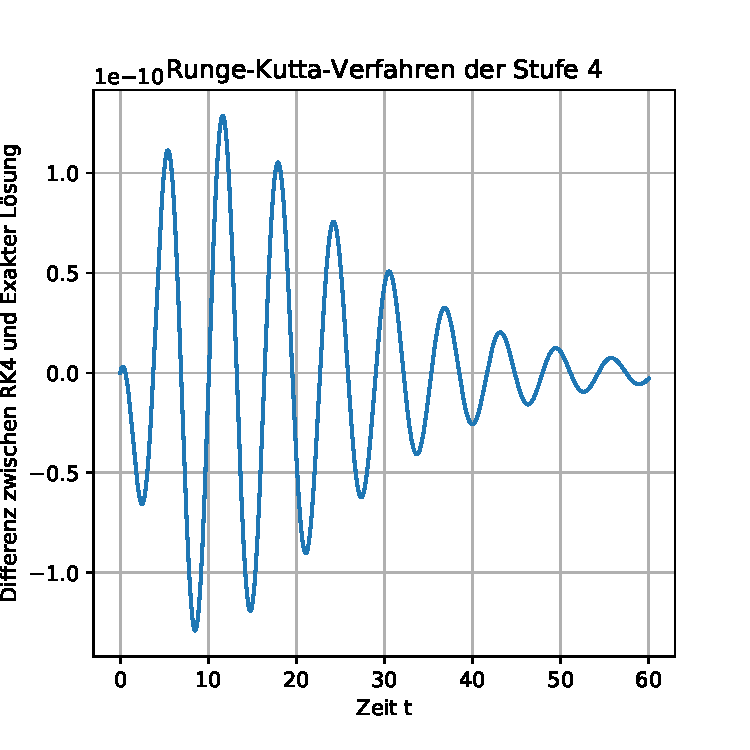
\includegraphics[width=0.8\textwidth]{Runge_Kutta_Proof.pdf}
	\caption{Runge-Kutta-Verfahren der Stufe 4}\label{f:rk4}
\end{figure}
In der Abbildung lässt sich erkennen, dass die numerische Lösung für kleine Zeiten $t$ sehr nahe an der exakten Lösung ist und selbst für größere Werte von $t$ die Differenz sich in der Größenordnung $10^{-10}$ aufhält. Damit ist die Genauigkeit des Runge-Kutta-Verfahrens 4. Ordnung bestätigt. Die Fehler konvergieren sogar gegen $0$ für große $t$.

\subsection{Teilaufgabe 3 - Korrektheit von RK4}
Um das Runge-Kutta-Verfahren zu verifizieren, führen wir zunächst eine Taylorentwicklung der Funktion $\vec{y}(t)$. durch. Für einen einzelnen Teilschritt mit der Zeitdifferenz $h$ gilt dann:
\begin{equation}
	\vec{y}(t+h) = \vec{y}(t) + h\frac{d\vec{y}}{dt}(t) + \frac{h^2}{2}\frac{d^2\vec{y}}{dt^2} + \frac{h^3}{6}\frac{d^3\vec{y}}{dt^3} + \frac{h^4}{24}\frac{d^4\vec{y}}{dt^4} + \mathcal{O}(h^5)
\end{equation}
Da die Differentialgleichung linear mit konstanten Koeffizienten ist, können wir für die Ableitungen schreiben:
\begin{equation*}
	\frac{d^n\vec{y}(t)}{dt^n} = F^n*\vec{y}(t)
\end{equation*}
Mit der Matrix $F$. Wir können aus der Differentialgleichung ablesen, dass für die Matrix $F$ gilt:
\begin{equation*}
	F = \begin{pmatrix}
	0 & 1 \\ -\omega_0^2 & -2\gamma
	\end{pmatrix}
\end{equation*}
Zudem können wir die Iterationsvorschrift des Runge-Kutta-Verfahrens ansehen und diese dann Umformen. Wir erhalten:
\begin{equation}
	\vec{y}(t+h) = \vec{y}(t) + \frac{1}{6}[\vec{k_1} + 2\vec{k_2} + 2\vec{k_3} + \vec{k_4}]
\end{equation}
Dabei gilt für die Stützvektoren $\vec{k_i}$:
\begin{align*}
	\vec{k_1} &= h\vec{f}(t, \vec{y(t)}) \\
	\vec{k_2} &= h\vec{f}(t+h/2, \vec{y(t)}+\vec{k_1}/2) \\
	\vec{k_3} &= h\vec{f}(t+h/2, \vec{y(t)}+\vec{k_2}/2) \\
	\vec{k_4} &= h\vec{f}(t+h , \vec{y(t)} + \vec{k_3})
\end{align*}
Wenn wir darin nun einsetzen, dass gilt:
\begin{equation*}
	\vec{f}(t, \vec{y(t)}) = F*\vec{y(t)}
\end{equation*}
Können wir diese Terme nacheinander umformen und inneinander einsetzen. Wir erhalten dann schließlich:
\begin{align}
	\vec{k_1} &= hF*\vec{y(t)} \\
	\vec{k_2} &= hF*\left(\vec{y(t)} + \frac{h}{2}F\vec{y(t)}\right) \\
	\vec{k_3} &= hF*\left(\vec{y(t)} + \frac{h}{2}F*\left(\vec{y(t)} + \frac{h}{2}F*\vec{y(t)}\right)\right) \\
	\vec{k_4} &= hF*\left(\vec{y(t)} + hF*\left(\vec{y(t)}+\frac{h}{2}F*\left(\vec{y(t)} + \frac{h}{2}F*\vec{y(t)}\right)\right)\right)
\end{align}
Wenn wir diese Ausdrücke für $\vec{k_i}$ jetzt in die Iterationsvorschrift für das Runge-Kutta-Verfahren einsetzen, erhalten wir schließlich:
\begin{equation}
	\vec{y}(t+h) = \vec{y}(t) + hF*\vec{y}(t) + \frac{h^2}{2}F^2*\vec{y}(t) + \frac{h^3}{6}F^3*\vec{y}(t) + \frac{h^4}{24}F^4*\vec{y}(t)
\end{equation}
Wir sehen also, das das RK4-Verfahren bis auf eine Ordnung $\mathcal{O}(h^5)$ mit einer analytischen Lösung übereinstimmt. Damit haben wir es verifiziert.

Um den Spektralradius dieses Verfahrens zu berechnen, lesen wir zunächst die Vergrößerungsmatrix $G$ ab. Für $G$ gilt:
\begin{equation*}
	G = hF + \frac{h^2}{2}F^2 + \frac{h^3}{6}F^3 + \frac{h^4}{24}F^4
\end{equation*}
Und mit den angegebenen Werten für $\omega_0$ und $\gamma$ erhalten wir schließlich:
\begin{equation}
	G = \begin{pmatrix}
	-\frac{h^2}{2}+\frac{h^3}{30}+\frac{h^4}{25} & h-\frac{0,2h^2}{2} - \frac{0,96h^3}{6} + \frac{0,392h^4}{24}\\
	-h++\frac{0,2h^2}{2} + \frac{0,96h^3}{6} - \frac{0.392h^4}{24} & -0,2h-\frac{0,96h^2}{2} + \frac{0.392h^3}{6} + \frac{0.8816h^4}{24}
	\end{pmatrix}
\end{equation}
Die Eigenwerte dieser Matrix berechnen wir dann mit Mathematica. Wir erhalten:
\begin{align*}
	\lambda_{1,2} &=0.000868056 h [-564.48 h-115.2+44.1984 h^3+56.832 h^2 \\
	& \pm \sqrt{-350.501 h^6+6866.97 h^5-29342.3 h^4-84961.2 h^3+407288.h^2+262767. h-1.31383\times 10^6}]
\end{align*}
Wir sehen, dass gilt:
\begin{equation*}
	\lim_{h \to 0}\lambda_{1,2} = 0
\end{equation*}
Deswegen ist das RK4-Verfahren für klein gewählte $h$ stabil und konvergiert gegen die analytische Lösung. Leider ließ sich in Mathematica keine Ungleichung für $|\lambda_{1,2}| < 1$ lösen, insofern kann ich keine genauere Einschränkung für die Größe von $h$ vornehmen. Für den Spektralradius $\rho$ der Vergrößerungsmatrix gilt dann:
\begin{equation*}
	\rho(F) = \max|\lambda_{1,2}|
\end{equation*}


\section{Aufgabe  H5 - Kopplung an ein externes Feld}
\subsection{Teilaufgabe 1 - Implementierung}
Wir verändern jetzt unsere Differentialgleichung, da der  gedämpfte Oszillator nun durch ein externes Feld angeregt wird. Die neue Differentialgleichung lautet dann:
\begin{equation}
	\frac{d^2x}{dt^2}(t) = -\omega_0^2x(t) - 2\gamma\frac{dx}{dt}(t) + \alpha\cos(\omega t)
\end{equation}
Die Lösung dieser Gleichung setzt sich aus einem homogenen und partikulären Teil zusammen. Wir wählen wieder als Ansatz:
\begin{align}
	x_{homogen}(t) &= e^{-\gamma t}\left[A\cos(\omega't)+B\sin(\omega't)\right] \\
	x_{inhomogen}(t) &= C\cos(\omega t) + D\sin(\omega t)
\end{align}
Zunächst lösen wir den inhomogen Teil, sodass $C$ und $D$ die Differentialgleichung erfüllen. Wir erhalten dann:
\begin{align*}
	C &= \frac{\alpha(\omega_0^2 - \omega^2)}{(\omega_0^2 - \omega^2)^2+ 4\gamma^2\omega^2} \\
	D &= \frac{2\gamma\alpha\omega}{(\omega_0^2 - \omega^2)^2+ 4\gamma^2\omega^2}
\end{align*}
Jetzt können wir unseren Ansatz für den homogenen Teil einsetzen und $A$ und $B$ bestimmen, sodass die Anfangsbedingungen erfüllt sind.  Wir erhalten dann als Werte:
\begin{align*}
	A &= x_0 - \frac{\alpha (\omega_0^2 -\omega^2)}{(\omega_0^2 - \omega^2)^2+ 4\gamma^2\omega^2} \\
	B &= \frac{v_0}{\omega'} + \frac{\gamma A}{\omega'} - \frac{2\gamma\alpha\omega^2}{((\omega_0^2 - \omega^2)^2+ 4\gamma^2\omega^2)\omega'}
\end{align*}
Dabei gilt $\omega' = \sqrt{\gamma^2 -\omega_0^2}$.
\subsection{Teilaufgabe 2 - Verifizierung}
Mit dieser Funktion können wir wieder die Genauigkeit des Verfahrens testen. Die Differenzen zwischen analytischer und numerischer Lösungen sehen wir in Abbildung \ref{f:extFeld}.
\begin{figure}[htbp]
	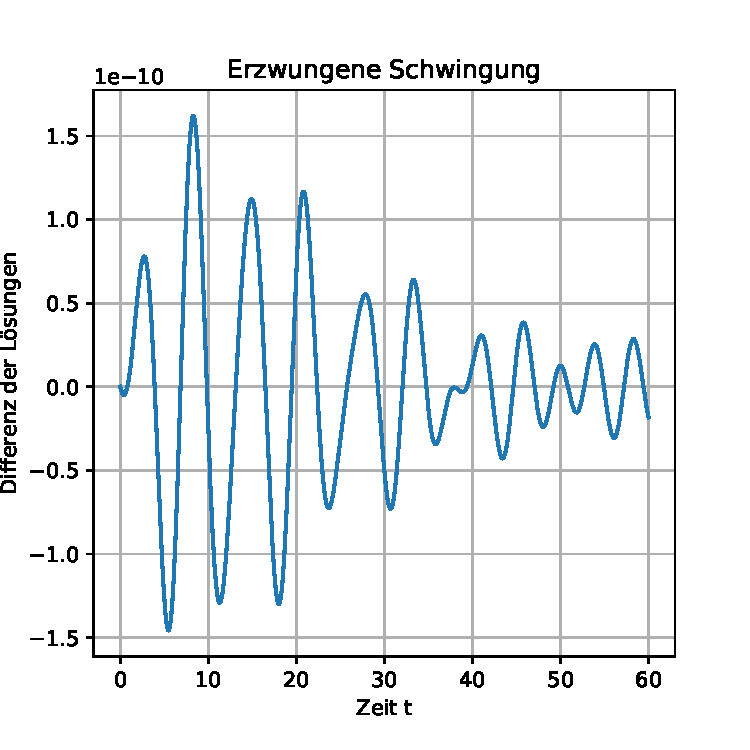
\includegraphics[width=0.8\textwidth]{Erzwungene_Schwingung.pdf}
	\caption[Erzwungene Schwingung]{Fehler der Numerischen Simulation der erzwungenen Schwingung}\label{f:extFeld}
\end{figure}
Auch hier sehen wir wieder, dass die Werte zu Beginn sehr nahe bei einander liegen und  auch für größere $t$  der Fehler immer noch in der  Größenordnung $10^{-10}$  ist. Damit ist dieses Verfahren auch für eine erzwungene Schwingung sehr genau und wir  können in der nächsten Aufgabe auch eine  Frequenzanalyse für viele Perioden durchführen.

\section{Aufgabe H6 - Tune in}
\subsection{Teilaufgabe 1 - Implementierung}
Wir führen jetzt eine Frequenzanalyse für eine unbekannte externe Kraft durch. Dazu modifizieren wir zunächst unsere Differentialgleichung zu:
\begin{equation}
	\frac{d^2x}{dt^2}(t) = -\omega_0^2x(t) - 2\gamma\frac{dx}{dt}(t) + f_{ext}(t)
\end{equation}
Wir können die neue Bahnkurve auch anzeigen. Diese sieht man in Abbildung \ref{f:Kraft_unknown}.
\begin{figure}
	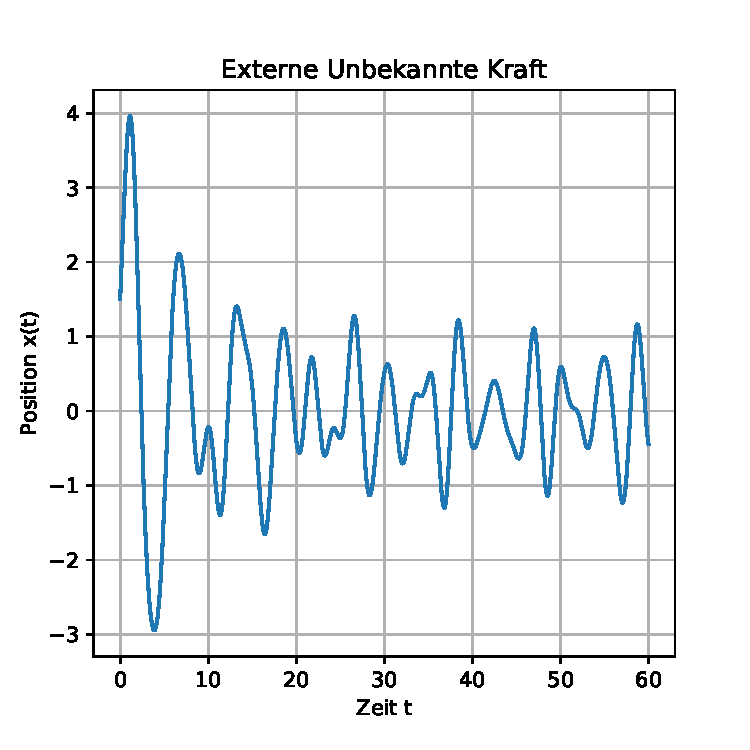
\includegraphics[width=0.8\textwidth]{unbekannteKraft.pdf}
	\caption{Bahnkurve mit unbekannter externer Kraft}\label{f:Kraft_unknown}
\end{figure}
Man erkennt sehr gut, wie zunächst die sinusförmige, abfallende Schwingung wie in Aufgabe H4 und H5 überwiegt, aber ab etwa $t=7.5$ ist die ursprüngliche Schwingung sehr stark abgefallen, sodass die externe Anregung überwiegt und das System in eine nicht harmonische Bewegung zwingt.

\subsection{Teilaufgabe 2 - Durchschnittliche Leistung}
Wir haben aus der Implementierung nun die Bahnkurve extrahiert, wir können aber auch die Momentangeschwindigkeit numerisch bestimmen und damit die Leistung des Systems bestimmen. Für diese Leistung gilt:
\begin{equation*}
	P(t) = f_{ext}(t)\dot{x}(t)
\end{equation*}
Daraus können wir die durchschnittliche Leistung einer Periode bestimmen durch:
\begin{equation*}
	\overline{P(t)} = \frac{1}{T}\int_{t_1}^{t_1+T}P(t)dt
\end{equation*}
Die Periode $T$ einer Schwingung können wir dabei durch $T = 2\pi\omega_0$ bestimmen. Damit können wir für eine beliebige Anzahl an Perioden die durchschnittliche Leistung bestimmen, da das RK4-Verfahren auch für große Zeiten $t$ stabil ist. Um das Integral zu berechnen benutzen wir das Trapez-Verfahren. In  Abbildung \ref{f:power_avg} sehen wir die durchschnittliche Leistung der ersten zwölf Perioden mit $\omega_0=1$.
\begin{figure}
	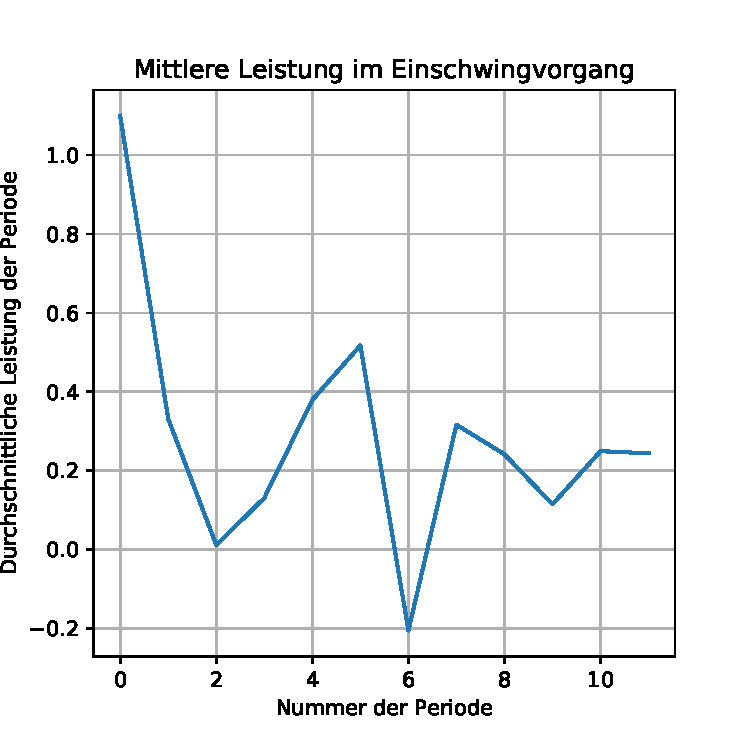
\includegraphics[width=0.8\textwidth]{Einschwing.pdf}
	\caption{Durchschnittliche Leistung}\label{f:power_avg}
\end{figure}
\subsection{Teilaufgabe 3 - Scan in $\omega_0$}

Wir führen nun einen Scan in $\omega_0$ durch. Dafür variieren wir $\omega_0$ zwischen 1 und 3 und berechnen die durchschnittliche Leistung $\overline{P(t)}$ der ersten 60 Perioden und daraus die durchschnittliche Leistung $\overline{P(\omega_0)}$ für die ersten 60 Perioden. Das Resultat sehen wir in Abbildung \ref{f:power_scan}.
\begin{figure}
	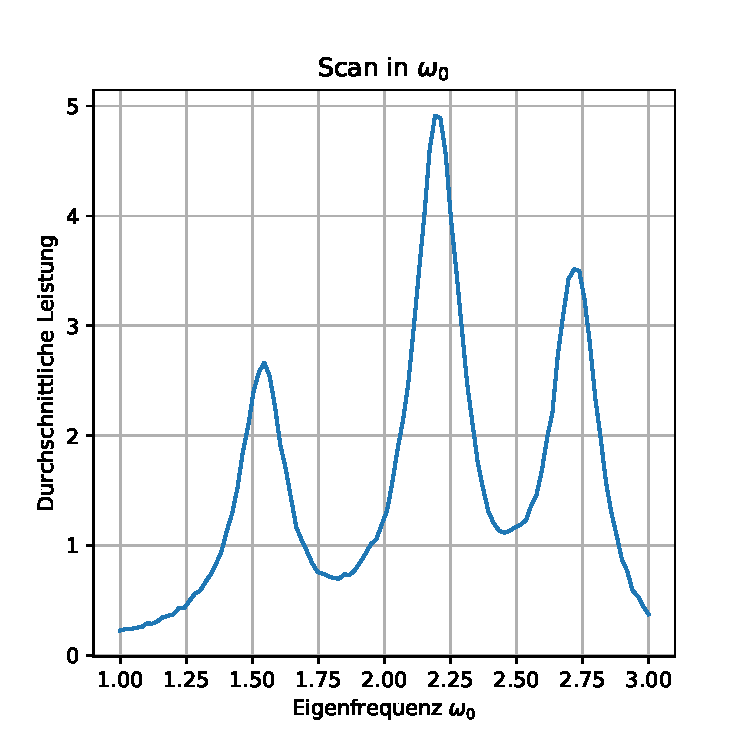
\includegraphics{Scan_Omega_Power.pdf}
	\caption{Leistungsverlauf in Abhängigkeit von $\omega_0$}\label{f:power_scan}
\end{figure}
Wir sehen drei ausgeprägte Peaks in dem Leistungsverlauf zwischen $\omega_0=1$ und $\omega_0=3$. Dies lässt darauf schließen, dass die anregende Funktion $f_{ext}(t)$ ebenfalls drei Eigenfrequenzen besitzt, mit denen diese schwingt. Mit einer solchen Analyse kann man also eine externe Funktion in ihre Frequenzkomponenten zerlegen, also eine Art Fourieranalyse. Dies passiert, da die Leistung maximal wird, wenn die Eigenfrequenz und die Anregerfrequenz sehr nahe beieinander sind. Dies ist das gleiche Konzept wie bei einer Resonanzkatastrophe, allerdings nutzen wir dieses hier, um die unbekannte Funktion in ihre Frequenzanteile zu zerlegen.
\newpage
\listoffigures
\end{document}